\documentclass[conference]{IEEEtran}

\usepackage{times}
\usepackage{amsmath}
\usepackage{booktabs}
\usepackage{hyperref}
\usepackage{xspace}
\usepackage{tikz}
\usetikzlibrary{positioning,arrows.meta}
\usepackage{pgfplots}
\pgfplotsset{compat=1.17}

\hyphenation{op-tical net-works semi-conduc-tor}

\newcommand{\nomic}{\texttt{nomic-embed-text-v1.5}\xspace}
\newcommand{\HR}[1]{\mathrm{HR}@{#1}}
\newcommand{\MRR}[1]{\mathrm{MRR}@{#1}}
\newcommand{\NDCG}[1]{\mathrm{NDCG}@{#1}}

\begin{document}

\title{Evaluating Hybrid Sparse-Dense Retrieval\\
for EU Climate Legal Documents}

\author{
  \IEEEauthorblockN{Rameez Wani}
  \IEEEauthorblockA{School of Computing\\
    Dublin City University\\
    Dublin, Ireland\\
    rameezshafat.wani2@mail.dcu.ie}
  \and
  \IEEEauthorblockN{Ananya Warior}
  \IEEEauthorblockA{School of Computing\\
    Dublin City University\\
    Dublin, Ireland\\
    ananyasalil.warior2@mail.dcu.ie}
}

\maketitle

\begin{abstract}
Legal information retrieval in statutory corpora poses specific
challenges due to formulaic language, hierarchical authority structures,
and the need for doctrinal precision.
This paper evaluates three first-stage retrieval configurations---BM25
lexical search, \nomic dense retrieval (768-dim,
8{,}192-token context), and a hybrid combining both via weighted
Reciprocal Rank Fusion (RRF, $k{=}20$, dense weight~5)---on a
102-query benchmark over EU Climate Law, of which 31~test queries are
derived from real written questions submitted by Members of the
European Parliament, providing externally sourced information needs
that control against query--corpus vocabulary leakage.
The corpus comprises 1{,}156 article-level provisions (1{,}166
retrieval units after splitting oversized amendment articles)
extracted from 72~EU legislative instruments via SPARQL and
Formex~XML.
Fusion parameters were tuned on a 49-query validation split; all
reported metrics are from the sealed 53-query test set.
Dense retrieval achieves $\HR{5}{=}0.925$, substantially outperforming
BM25 ($\HR{5}{=}0.698$; Wilcoxon $p{=}0.004$).
The hybrid achieves $\HR{5}{=}0.906$, $\MRR{5}{=}0.773$, and
$\NDCG{5}{=}0.721$, the highest MRR and NDCG of all three systems,
but its improvement over dense alone is statistically non-significant
($p{=}0.614$).
Only 5 of 53 queries ($9.4\,\%$) are hard failures for the hybrid.
A paired experiment re-evaluating 71~identical information needs
under their original corpus-derived wording shows why leakage control
matters: reworded queries cost BM25 $0.29$ of $\MRR{5}$ but the dense
retriever only $0.09$, meaning leaky benchmarks manufacture a false
parity between lexical and semantic retrieval.
The results confirm that a strong general-domain dense retriever
already approaches ceiling performance on this corpus, and that
weighted lexical-semantic fusion provides consistent ranking gains
without statistically significant coverage improvement.
\end{abstract}

\begin{IEEEkeywords}
Legal Information Retrieval, Hybrid Retrieval, BM25,
Dense Retrieval, Reciprocal Rank Fusion, EU Climate Law,
Retrieval-Augmented Generation, Statute-Level Benchmark
\end{IEEEkeywords}

\IEEEpeerreviewmaketitle

% ============================================================
\section{Introduction}

Anyone who has tried to answer a legal question from primary
legislation knows that finding the right document is most of the
battle.
The meaning of law depends on exact wording, cross-references, and
which of several similar-sounding instruments actually governs the
situation at hand.
EU climate and energy law makes this unusually difficult: the
Emissions Trading System directive of 2003 has been amended repeatedly,
the Carbon Border Adjustment Mechanism borrows its allowance
definitions from that directive, and dozens of implementing and
delegated acts reuse the same vocabulary---\textit{free allocation},
\textit{carbon leakage}, \textit{monitoring and reporting}---for
legally distinct obligations.
A retrieval system that returns a plausible but wrong instrument does
not produce an approximate answer; it produces the wrong law.
The stakes are highest in retrieval-augmented generation (RAG)
pipelines, where the first-stage retriever determines whether
citation-grounded generation is possible at all~\cite{14}.
This paper evaluates that first stage.

The standard tension in legal retrieval is between lexical and
semantic matching.
BM25 performs well on formulaic legal text, where exact term overlap
is a strong relevance signal~\cite{1}, but a compliance officer asking
whether her shipping company ``has to pay for the pollution its
vessels cause'' shares almost no vocabulary with a provision on
``surrender requirements in respect of maritime transport
activities'' (Directive~2023/959).
Dense retrievers bridge that vocabulary gap, but bring failure modes
of their own: semantically similar passages from the wrong instrument
can rank highly because legal drafting recycles structural
boilerplate~\cite{12}, and off-the-shelf embedding models often
degrade on specialised corpora~\cite{14}.
Hybrid sparse--dense fusion is the commonly recommended
remedy~\cite{2,3,10}.
Whether that recommendation holds for statute-level retrieval over a
small, terminologically dense corpus is, however, an empirical
question---and answering it fairly turned out to be harder than
building the systems.

Our first evaluation attempt taught us why.
In a pilot benchmark whose queries were written while consulting the
corpus, every configuration looked excellent and the hybrid appeared
to win outright; the strongest system reached a perfect hit rate.
The queries had simply inherited the statutes' vocabulary, so the
benchmark was rewarding term overlap rather than retrieval quality,
flattering BM25 in particular.
We therefore rebuilt the benchmark under an explicit leakage-control
protocol: every query was rewritten in the plain language of a
non-expert, and the test set was extended with queries derived from
written parliamentary questions that Members of the European
Parliament submitted to the Commission---real information needs,
documented by their parliamentary reference numbers, whose official
answers often name the very instruments a correct retrieval should
return.
To our knowledge, no prior work on hybrid legal retrieval has
evaluated statute-level EU climate law, and none has controlled for
query--corpus vocabulary leakage in this way.

We ask two questions.
\textbf{RQ1.} Does hybrid sparse--dense retrieval improve
effectiveness and reliability over BM25-only and dense-only baselines
for EU Climate Law statute retrieval?
\textbf{RQ2.} What failure modes remain for the strongest
configuration, and do they indicate that first-stage retrieval is the
bottleneck for grounded legal RAG in this domain?

Our contributions are:
(i)~a 102-query benchmark for statute-level EU Climate Law retrieval
with binary CELEX-level relevance judgements and a sealed 53-query
test set, constructed under the leakage-control protocol above, with
31~test queries traceable to documented European Parliament written
questions;
(ii)~a reproducible corpus of 1{,}156 article-level provisions from
72~EU climate instruments, extracted through a documented two-phase
SPARQL pipeline over the CELLAR repository; and
(iii)~a three-way comparison of BM25, a pure dense bi-encoder, and
weighted reciprocal rank fusion, with bootstrap confidence intervals,
significance testing, and per-query failure analysis.

To preview the results: on the leakage-controlled test set, both the
dense retriever and the hybrid significantly outperform BM25, but the
hybrid is statistically indistinguishable from the dense retriever
alone, and the direction of that comparison reversed as the test set
grew---a caution against reading small-sample differences between
strong systems.
The remaining failures are ranking errors on provisions buried inside
large amending instruments, not gaps in corpus coverage, which points
to corpus preprocessing rather than retrieval strategy as the next
lever for improvement.

The remainder of this paper is structured as follows.
Section~II reviews related work on lexical, dense, and hybrid legal
retrieval.
Section~III describes the system: corpus construction, the two
retrievers, and the fusion method.
Section~IV details the benchmark construction protocol, metrics, and
experimental configuration.
Section~V presents results, including significance testing and
per-query failure analysis; Section~VI discusses their implications;
and Section~VII concludes with limitations and future work.

% ============================================================
\section{Related Work}

\subsection{Lexical vs.\ Dense Retrieval in Legal IR}

Mori et al.~\cite{1} demonstrate that BM25 remains a competitive
baseline for formulaic legal texts where exact term overlap is a
reliable relevance signal.
Dense models tend to underperform in such settings because semantic
similarity ignores legally binding phrasing.
Conversely, Zheng et al.~\cite{8} show that lexical models degrade on
reasoning-intensive queries; semantic models handle analogical
reasoning more effectively.
The LRAGE evaluation framework~\cite{14} confirms that off-the-shelf
dense retrievers underperform BM25 on legal retrieval tasks without
domain-specific adaptation.

\subsection{Hybrid Retrieval}

Rayo et al.~\cite{3} show that combining BM25 with fine-tuned sentence
transformers substantially improves Recall@10 and MAP@10 on regulatory
corpora.
LegalRAG~\cite{10} demonstrates that hybrid systems outperform
single-mode systems for multilingual legal texts.
HyPA-RAG~\cite{2} introduces adaptive parameter adjustment for hybrid
retrieval in AI legal and policy applications.
SPLADE~\cite{5} and its efficiency-optimised variant~\cite{4} provide
sparse learned representations that address vocabulary mismatch while
maintaining inverted-index compatibility.

\subsection{Retrieval Reliability and Legal RAG}

Reuter et al.~\cite{12} identify Document-Level Retrieval Mismatch
(DRM) as a systematic failure mode of dense retrievers on large legal
datasets, where shared structural boilerplate causes globally
irrelevant documents to rank highly.
Ho et al.~\cite{13} show that doctrinal accuracy requires structural
legal signals beyond semantic similarity.
CBR-RAG~\cite{6} and LexRAG~\cite{7} demonstrate that multi-turn
legal grounding requires retrieval robust to topic drift and implicit
definitional dependencies.
Multi-stage architectures combining embedding models with LLM
re-ranking have proven effective in the COLIEE legal retrieval
competition~\cite{11}, and LexDrafter~\cite{9} applies
retrieval-augmented generation directly to EU legislative documents
for terminology drafting---the closest prior work to our corpus
domain, though it does not evaluate first-stage retrieval quality.

% ============================================================
\section{System Architecture}

Fig.~\ref{fig:arch} shows the end-to-end pipeline: corpus
construction from CELLAR, dual indexing, and query-time fusion.

\begin{figure}[!t]
\centering
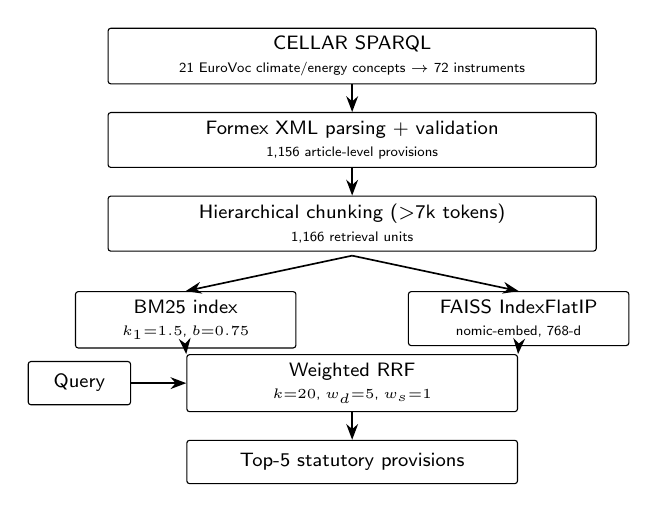
\begin{tikzpicture}[
  node distance=3.5mm and 4mm,
  box/.style={draw, rounded corners=1pt, align=center,
              font=\scriptsize\sffamily, inner sep=3pt,
              minimum height=5.5mm},
  arr/.style={-{Stealth[length=2mm]}, semithick}
]
\node[box, minimum width=62mm] (cellar)
  {CELLAR SPARQL\\ \tiny 21 EuroVoc climate/energy concepts $\rightarrow$ 72 instruments};
\node[box, minimum width=62mm, below=of cellar] (formex)
  {Formex XML parsing + validation\\ \tiny 1{,}156 article-level provisions};
\node[box, minimum width=62mm, below=of formex] (chunk)
  {Hierarchical chunking ($>$7k tokens)\\ \tiny 1{,}166 retrieval units};
\node[box, below left=5mm and -24mm of chunk, minimum width=28mm] (bm25)
  {BM25 index\\ \tiny $k_1{=}1.5$, $b{=}0.75$};
\node[box, below right=5mm and -24mm of chunk, minimum width=28mm] (faiss)
  {FAISS IndexFlatIP\\ \tiny nomic-embed, 768-d};
\node[box, below=13mm of chunk, minimum width=42mm] (rrf)
  {Weighted RRF\\ \tiny $k{=}20$, $w_d{=}5$, $w_s{=}1$};
\node[box, below=of rrf, minimum width=42mm] (out)
  {Top-5 statutory provisions};
\node[box, left=7mm of rrf, minimum width=13mm] (query) {Query};

\draw[arr] (cellar) -- (formex);
\draw[arr] (formex) -- (chunk);
\draw[arr] (chunk.south) ++(0,-0.5mm) -- (bm25.north);
\draw[arr] (chunk.south) ++(0,-0.5mm) -- (faiss.north);
\draw[arr] (bm25.south) -- (rrf.north west);
\draw[arr] (faiss.south) -- (rrf.north east);
\draw[arr] (query) -- (rrf);
\draw[arr] (rrf) -- (out);
\end{tikzpicture}
\caption{System pipeline: two-phase CELLAR extraction, dual
sparse/dense indexing over 1{,}166 retrieval units, and query-time
weighted reciprocal rank fusion. Both retrievers return their top-100
candidates concurrently.}
\label{fig:arch}
\end{figure}

\subsection{Corpus Construction}

We extract the corpus from the EU CELLAR repository in two phases.
A SPARQL query first retrieves every work URI associated with any of
21~EuroVoc climate and energy concept identifiers, which yields the
72~instruments; per-document manifestation queries then resolve the
Formex~XML (\texttt{fmx4}) download URL for each instrument, falling
back to the HTML manifestation for the few documents that lack one.
Formex is the Publications Office's structured drafting format, so
parsing it (with \texttt{lxml}) recovers the legal structure of each
act directly instead of reverse-engineering it from rendered HTML.

The retrieval unit is the legislative article.
This is a deliberate choice rather than a convenience: EU articles
are drafted as self-contained units---each states one obligation,
definition, or procedure---so they align with what a legal user
actually needs retrieved, and they spare us the arbitrary window-size
decisions of token-based chunking.
Concretely, each \texttt{<ARTICLE>} element becomes one unit, with
text reconstructed from \texttt{<ALINEA>} leaf nodes to avoid
duplicated nesting; every record is validated against a schema, and
placeholder articles are discarded.
The exception is amending instruments, whose Article~1 can run to
tens of thousands of tokens because it contains every amendment the
act makes.
Five such articles exceed a 7{,}000-token limit (chosen to leave
headroom below the dense encoder's 8{,}192-token window) and are
split at the natural amendment-point boundaries; the resulting
sub-chunks inherit the parent \texttt{celex\_id}, so retrieval
results always resolve to a citable instrument.

The final corpus contains \textbf{1{,}156} article-level provisions
(\textbf{1{,}166} retrieval units after splitting) from
\textbf{72}~CELEX instruments covering ETS, CBAM, Taxonomy,
LULUCF, F-Gas, Maritime MRV, ESR, the European Climate Law, Energy
Efficiency, CSDDD, and the Governance Regulation.

\subsection{Sparse Retrieval --- BM25}

The lexical retriever is BM25Okapi~\cite{16}
(\texttt{rank-bm25}~0.2.2) with the standard parameters $k_1{=}1.5$
and $b{=}0.75$.
The only customisation is the tokeniser, which is built for statutory
text: hyphenated terms of art such as \textit{net-zero} survive as
single tokens, and we apply neither stemming nor stopword removal.
Both omissions are intentional.
EU definitions are terminologically precise---\textit{allowance} and
\textit{allowances} can appear in differently scoped provisions---and
stopword removal would break fixed legal phrases such as \textit{free
of charge} and \textit{not later than}, whose function words carry
the legal meaning.
At query time BM25 scores all 1{,}166 units and returns the top~100.

\subsection{Dense Retrieval --- nomic-embed-text-v1.5}

The semantic retriever is \nomic~\cite{17}, a 768-dimensional
bi-encoder with an 8{,}192-token context window, loaded via
\texttt{sentence-transformers}.
Three properties drove the selection.
It is fully open-weight, which keeps the pipeline reproducible
without API access.
Its long context window embeds EU articles whole---only the five
oversized amendment articles described above need splitting---where a
conventional 512-token encoder would silently truncate roughly a
fifth of this corpus.
Most importantly for the experimental design, it is a \emph{pure}
bi-encoder: models trained jointly for dense, sparse, and
late-interaction retrieval (such as BGE-M3) already encode lexical
signals in their dense vectors, which would muddy any conclusion
about what BM25 adds on top.

Following the model's asymmetric training scheme, queries are
prefixed with \texttt{"search\_query:"} and articles with
\texttt{"search\_document:"} before encoding.
Corpus vectors are L2-normalised and stored in a FAISS~\cite{18}
\texttt{IndexFlatIP}, where inner product on normalised vectors
equals cosine similarity; at 1{,}166 vectors, exact search is
trivially fast and no approximate index is needed.
At query time, FAISS returns the top~100 nearest neighbours.

\subsection{Reciprocal Rank Fusion}

Both retrievers run concurrently on each query
(\texttt{ThreadPool\-Executor}, two workers), and their ranked lists
are merged by weighted Reciprocal Rank Fusion~\cite{15}.
Each candidate document~$d$ receives the score

\begin{equation}
  \mathrm{RRF}(d) = \frac{w_s}{k + \mathrm{rank}_s(d)}
                  + \frac{w_d}{k + \mathrm{rank}_d(d)}
  \label{eq:rrf}
\end{equation}

\noindent where $\mathrm{rank}_s$ and $\mathrm{rank}_d$ are the
document's positions in the sparse and dense lists
($\infty$ if absent), $k$ dampens the influence of any single
top-ranked result, and $w_s$, $w_d$ weight the two retrievers.
The intuition of~\eqref{eq:rrf} is that a document ranked well by
both retrievers should beat a document ranked first by only one; the
weights let a systematically stronger retriever dominate ties.
The top~5 fused results form the system's output (and, in a full RAG
deployment, the context passed to generation).

We fuse ranks rather than raw scores because the two score scales are
incompatible: BM25 produces unbounded positive reals while cosine
similarity lies in $[-1,1]$, and any direct combination smuggles in
scale assumptions that rank-based fusion avoids
entirely~\cite{15}.
The operating point $k{=}20$, $w_s{=}1$, $w_d{=}5$ was chosen by grid
search on the 49-query validation split; the sealed 53-query test set
was evaluated only after these values were frozen.
Fig.~\ref{fig:sweep} shows the validation landscape: ranking quality
improves as the dense retriever is up-weighted, degrades sharply at
large~$k$, and the deployed configuration is the highest-MRR cell
among those reaching $\HR{5}{=}1.000$ on validation.

\begin{figure}[!t]
\centering
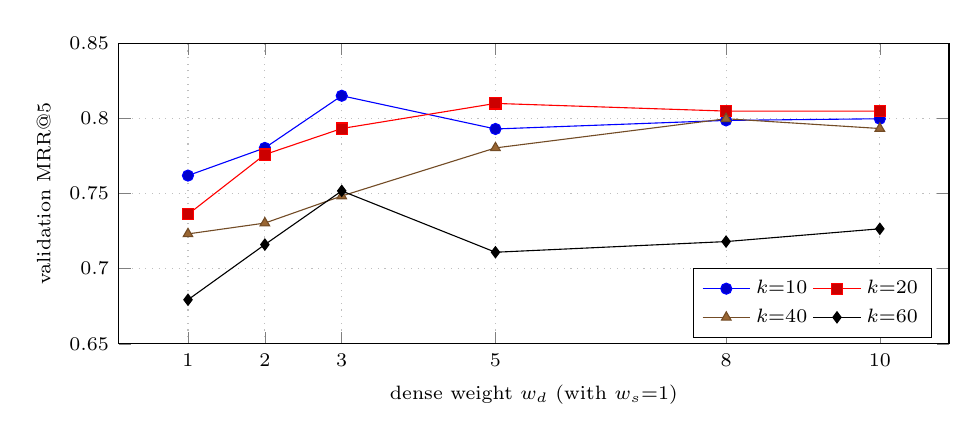
\begin{tikzpicture}
\begin{axis}[
  width=\columnwidth, height=54mm,
  xlabel={dense weight $w_d$ (with $w_s{=}1$)},
  ylabel={validation $\MRR{5}$},
  xtick={1,2,3,5,8,10},
  ymin=0.65, ymax=0.85,
  legend style={font=\scriptsize, at={(0.98,0.02)},
                anchor=south east, legend columns=2},
  tick label style={font=\scriptsize},
  label style={font=\scriptsize},
  grid=major, grid style={dotted}
]
\addplot+[mark=*] coordinates
  {(1,0.7619) (2,0.7803) (3,0.8150) (5,0.7929) (8,0.7986) (10,0.7997)};
\addplot+[mark=square*] coordinates
  {(1,0.7361) (2,0.7759) (3,0.7932) (5,0.8099) (8,0.8048) (10,0.8048)};
\addplot+[mark=triangle*] coordinates
  {(1,0.7231) (2,0.7303) (3,0.7483) (5,0.7803) (8,0.7997) (10,0.7932)};
\addplot+[mark=diamond*] coordinates
  {(1,0.6793) (2,0.7160) (3,0.7517) (5,0.7109) (8,0.7180) (10,0.7265)};
\legend{$k{=}10$,$k{=}20$,$k{=}40$,$k{=}60$}
\end{axis}
\end{tikzpicture}
\caption{Validation-split $\MRR{5}$ across the RRF grid.
The deployed configuration ($k{=}20$, $w_d{=}5$; $\MRR{5}{=}0.810$)
is the best-ranking cell that also achieves $\HR{5}{=}1.000$.
The literature-default region ($k{=}60$, low $w_d$, bottom-left)
performs worst.}
\label{fig:sweep}
\end{figure}

% ============================================================
\section{Experimental Setup}

\subsection{Benchmark}

The benchmark contains 102~queries covering all eleven EU Climate Law
instrument families, constructed in two stages.
An initial set of 71~queries was written in deliberately natural,
non-statutory language: an early pilot in which queries paraphrased
corpus wording produced near-perfect scores for all systems
($\HR{5}{=}1.0$), indicating query--corpus vocabulary leakage rather
than retrieval quality; all queries were therefore rewritten to
express the underlying information need without reusing statutory
vocabulary.
These 71~queries were split 70/30 by stratified difficulty (seed~42)
into a 49-query validation set (used exclusively for fusion-parameter
tuning) and a 22-query test set.
The test set was subsequently expanded with 31~queries derived from
written questions submitted by Members of the European Parliament to
the Commission: each parliamentary question was screened for
answerability from legislation, paraphrased into plain language, and
mapped to its relevant CELEX instruments, with the parliamentary
reference number (e.g., E-002271/2024) recorded per query as an audit
trail.
In many cases the Commission's official answer cites the relevant
instruments, providing independent corroboration of the relevance
judgement.
Corpus membership was verified for every mapping before a query was
accepted, so no query requires an instrument absent from the corpus.
All reported results use the resulting sealed \textbf{53-query test
set}; the validation set was never evaluated against reported metrics.
To give a flavour of the derivation: parliamentary question
E-004153/2025 asks whether a ship calling at a mainland port en route
to an outermost region owes allowances for the first leg of the
voyage; this becomes the plain-language query \emph{``A ship sails
from the mainland, stops at another mainland port, then continues to
one of the EU's remote overseas regions---is the whole journey spared
the carbon charge, or only the last leg?''}, mapped to
Directive~2023/959, whose derogation the Commission's answer cites.

Each query carries a difficulty tag used for stratification:
\emph{hard} queries share essentially no vocabulary with the statutory
text (e.g., ``the don't-make-anything-else-worse test'' for the
Taxonomy's \emph{do no significant harm} principle), while
\emph{standard} queries are naturally phrased but moderately
terminological.
Table~\ref{tab:benchmark} summarises the composition.
Relevance judgements target 62 of the 72 corpus instruments; the ten
never used as targets are annex-replacement amendment acts with no
self-contained content, excluded as relevance targets by
construction.

\begin{table}[!t]
\renewcommand{\arraystretch}{1.3}
\caption{Benchmark composition. ``$\geq$2 rel.''\ counts queries with
  two or more relevant instruments; ``instr.''\ counts distinct
  instruments used as relevance targets.}
\label{tab:benchmark}
\centering
\small
\begin{tabular}{@{}lccccc@{}}
\toprule
Subset & $n$ & standard & hard & $\geq$2 rel. & instr. \\
\midrule
Validation            &  49 & 36 & 13 & 29 & 44 \\
Test (original split) &  22 & 16 &  6 &  9 & 26 \\
Test (EP-derived)     &  31 & 19 & 12 & 13 & 22 \\
\midrule
Test (total)          &  53 & 35 & 18 & 22 & 37 \\
All queries           & 102 & 71 & 31 & 51 & 62 \\
\bottomrule
\end{tabular}
\end{table}

Relevance is binary at the CELEX instrument level: a document is
relevant if it contains the provision that directly and materially
answers the query.
CELEX identifiers with corrigendum suffixes (e.g.,
\texttt{32003L0087R(02)}) are normalised by stripping the
\texttt{R(...)} suffix before matching.

\subsection{Metrics}

We report three metrics at cut-off~5, matching the number of
provisions a downstream RAG stage would receive as context.
$\HR{5}$ measures coverage: the fraction of queries for which at
least one relevant instrument appears in the top~5 at all.
For grounded generation this is the make-or-break number---a miss
here cannot be repaired downstream.
$\MRR{5}$ measures how high the first relevant result lands, which
matters because generation quality degrades when the correct
provision sits below distractors.
$\NDCG{5}$ credits finding \emph{all} relevant instruments, not just
the first: 22 of the 53 test queries have two or more relevant
instruments (Table~\ref{tab:benchmark}), and MRR is blind to
everything after the first hit.
Gains are binary, and because retrieval is article-level---so several
articles of the same instrument can occupy the top~5---each relevant
instrument is credited once, at its highest-ranked occurrence;
crediting duplicates would inflate NDCG above~1.

With only 53 test queries, point estimates alone would be easy to
over-read, so we quantify uncertainty twice.
95\,\% confidence intervals are estimated by percentile bootstrap
over queries (5{,}000 resamples, seed~42), which assumes nothing
about the score distribution.
Pairwise comparisons between systems use the Wilcoxon signed-rank
test on per-query MRR ($\alpha{=}0.05$, two-tailed, $n{=}53$)---a
paired, non-parametric test appropriate for skewed per-query
scores---and we report Cohen's~$d$ alongside $p$-values so that
effect sizes are visible even where significance is not reached.

\subsection{Hardware and Software}

All reported results were produced on a consumer laptop (AMD
Ryzen~7 5700U, CPU-only, Windows~11)---deliberately modest hardware,
since one claim of this work is that the full pipeline is
reproducible without GPUs or paid APIs.
The software stack is Python~3.14.2 with
\texttt{sentence-transformers}~5.5.1, \texttt{faiss-cpu}~1.14.2,
\texttt{rank-bm25}~0.2.2, and \texttt{pydantic}~2.13.4; all versions
are pinned in the repository, and the combined indices occupy under
10\,MB.

% ============================================================
\section{Results}

\subsection{Retrieval Effectiveness}

Table~\ref{tab:effectiveness} reports the main results on the
53-query test set; the question it answers is RQ1---whether fusion
buys anything over either retriever alone.

\begin{table}[!t]
\renewcommand{\arraystretch}{1.3}
\caption{Retrieval effectiveness on the 53-query test set.
  Bootstrap 95\,\% CIs in parentheses for $\HR{5}$.
  $^\dagger p{=}0.0005$ vs.\ BM25;
  $^\ddagger p{=}0.004$ vs.\ BM25.}
\label{tab:effectiveness}
\centering
\small
\begin{tabular}{@{}lccc@{}}
\toprule
System & $\HR{5}$ & $\MRR{5}$ & $\NDCG{5}$ \\
\midrule
BM25
  & 0.698 (0.566--0.811)
  & 0.528
  & 0.494 \\
\nomic
  & \textbf{0.925} (0.849--0.981)$^\ddagger$
  & 0.743
  & 0.709 \\
Hybrid RRF
  & 0.906 (0.811--0.981)$^\dagger$
  & \textbf{0.773}
  & \textbf{0.721} \\
\bottomrule
\end{tabular}
\end{table}

The clearest result is the gap to BM25.
Both semantic configurations outperform it by more than twenty points
of $\HR{5}$, and both differences are statistically significant:
hybrid vs.\ BM25 at $p{=}0.0005$ (Cohen's $d{=}0.579$, medium effect)
and dense vs.\ BM25 at $p{=}0.004$ ($d{=}0.433$, small effect).
On a leakage-controlled benchmark, lexical retrieval alone misses
roughly three queries in ten.

Between the two semantic configurations the picture is a statistical
tie.
Dense retrieval posts the best $\HR{5}$ (0.925 vs.\ 0.906) while the
hybrid posts the best $\MRR{5}$ (0.773 vs.\ 0.743) and $\NDCG{5}$
(0.721 vs.\ 0.709), but the Wilcoxon test finds no significant
difference ($p{=}0.614$, $d{=}0.120$, negligible), and the bootstrap
confidence intervals of the two systems overlap substantially on
every metric (e.g., $\MRR{5}$: hybrid $[0.666, 0.868]$ vs.\ dense
$[0.639, 0.836]$; $\NDCG{5}$: hybrid $[0.627, 0.842]$ vs.\ dense
$[0.621, 0.791]$).
The honest answer to RQ1 is therefore split: fusion delivers a
significant improvement over the lexical baseline, but no measurable
improvement over a strong dense retriever used alone.

\subsection{Effect of Query Difficulty}

Table~\ref{tab:difficulty} splits the test set by the difficulty tag
introduced in Section~IV: \emph{standard} queries are naturally
phrased but moderately terminological, while \emph{hard} queries
share essentially no vocabulary with the statutes.

\begin{table}[!t]
\renewcommand{\arraystretch}{1.3}
\caption{Results by query difficulty (standard $n{=}35$,
  hard $n{=}18$).}
\label{tab:difficulty}
\centering
\small
\begin{tabular}{@{}llccc@{}}
\toprule
System & Subset & $\HR{5}$ & $\MRR{5}$ & $\NDCG{5}$ \\
\midrule
BM25       & standard & 0.743 & 0.611 & 0.559 \\
           & hard     & 0.611 & 0.366 & 0.367 \\
\midrule
\nomic     & standard & 0.943 & 0.784 & 0.738 \\
           & hard     & 0.889 & 0.661 & 0.654 \\
\midrule
Hybrid RRF & standard & 0.943 & 0.821 & 0.754 \\
           & hard     & 0.833 & 0.680 & 0.655 \\
\bottomrule
\end{tabular}
\end{table}

The split localises exactly where lexical retrieval breaks.
On standard queries BM25 is usable ($\MRR{5}{=}0.611$); on hard
queries its $\MRR{5}$ nearly halves to 0.366, while dense retrieval
degrades far more gently (0.784 to 0.661).
The gap between the paradigms therefore \emph{widens} with vocabulary
mismatch---from 0.17 to 0.30 in $\MRR{5}$---which is the designed
purpose of the hard tier and direct evidence for the mechanism
claimed throughout: BM25's failure mode is vocabulary, not ranking.
The same split also explains where fusion helps at all: the hybrid's
$\MRR{5}$ advantage over dense is concentrated on standard queries
($+0.037$) and shrinks on hard ones ($+0.019$), consistent with
BM25's signal being trustworthy only when the query shares at least
some statutory vocabulary.

\subsection{Quantifying Vocabulary Leakage}

The pilot benchmark's original corpus-derived queries were preserved,
which permits a controlled experiment: the same 71~information needs,
with identical relevance judgements, evaluated under both their
original statutory wording and their leakage-controlled rewriting.
Nothing else varies---corpus, indices, and systems are held fixed.
Table~\ref{tab:leakage} reports the result.

\begin{table}[!t]
\renewcommand{\arraystretch}{1.3}
\caption{Paired leakage experiment: 71 identical information needs
  and relevance judgements under corpus-derived (leaky) versus
  plain-language (controlled) wording.}
\label{tab:leakage}
\centering
\small
\begin{tabular}{@{}lcccc@{}}
\toprule
& \multicolumn{2}{c}{Leaky wording}
& \multicolumn{2}{c}{Controlled wording} \\
\cmidrule(lr){2-3}\cmidrule(lr){4-5}
System & $\HR{5}$ & $\MRR{5}$ & $\HR{5}$ & $\MRR{5}$ \\
\midrule
BM25       & 0.958 & 0.846 & 0.704 & 0.556 \\
\nomic     & 0.986 & 0.870 & 0.958 & 0.785 \\
Hybrid RRF & 0.986 & 0.876 & 0.972 & 0.795 \\
\bottomrule
\end{tabular}
\end{table}

Under leaky wording, all three systems sit within three points of one
another and the benchmark cannot distinguish them.
Rewriting the queries costs BM25 $0.254$ of $\HR{5}$ and $0.290$ of
$\MRR{5}$, while the dense retriever loses only $0.028$ and $0.085$
respectively---leakage inflates lexical retrieval roughly three and a
half times more than semantic retrieval, manufacturing a parity that
does not survive realistic phrasing.
Two caveats: these 71~pairs include the 49~validation queries, so the
absolute values are not comparable with Table~\ref{tab:effectiveness}
and carry no held-out guarantee; and no tuning was performed on
either wording of this set beyond the validation use already
described.
The comparison is between wordings, not systems, and for that purpose
the pairing is exact.

\subsection{A Worked Example}

Table~\ref{tab:example} shows the actual top-5 lists for one hard
test query: \emph{``Is there any leeway in the EU's land-carbon rules
for a country whose forests get wrecked by wildfires or bark
beetles?''}
The relevant instruments are the LULUCF Regulation (2018/841) and its
2023 amendment (2023/839), whose flexibility provisions speak of
``natural disturbances''---none of the query's content words appears
in the statute.
With nothing lexical to anchor on, BM25 is confidently wrong across
two unrelated regimes, filling its list with the European Green Bond
Standard and CBAM instruments on the strength of incidental term
matches.
The dense retriever maps the paraphrase onto the natural-disturbance
provisions directly, placing both relevant instruments in its top
five; the dense-weighted fusion preserves them.

\begin{table}[!t]
\renewcommand{\arraystretch}{1.3}
\caption{Top-5 retrieved instruments for the wildfire/bark-beetle
  query. Relevant instruments in \textbf{bold}; repeated entries are
  different articles of the same instrument.}
\label{tab:example}
\centering
\scriptsize
\begin{tabular}{@{}clll@{}}
\toprule
Rank & BM25 & \nomic & Hybrid RRF \\
\midrule
1 & EuGB 2023/2631      & \textbf{LULUCF 2023/839} & \textbf{LULUCF 2023/839} \\
2 & CBAM am.\ 2025/2083 & \textbf{LULUCF 2023/839} & \textbf{LULUCF 2023/839} \\
3 & CBAM 2023/956       & \textbf{LULUCF 2018/841} & Nat.\ Rest.\ 2024/1991 \\
4 & CBAM 2023/956       & Nat.\ Rest.\ 2024/1991   & \textbf{LULUCF 2018/841} \\
5 & EuGB 2023/2631      & \textbf{LULUCF 2018/841} & \textbf{LULUCF 2018/841} \\
\bottomrule
\end{tabular}
\end{table}

\subsection{Hard Failure Analysis}

RQ2 asks what failures remain; Table~\ref{tab:reliability} breaks
down per-query outcomes across the three systems.

\begin{table}[!t]
\renewcommand{\arraystretch}{1.3}
\caption{Per-query hit pattern breakdown ($n{=}53$).}
\label{tab:reliability}
\centering
\small
\begin{tabular}{@{}lcc@{}}
\toprule
Category & $n$ & Fraction \\
\midrule
All three systems hit               & 36 & 0.679 \\
Dense and hybrid hit; BM25 misses   & 12 & 0.226 \\
Only BM25 hits                      &  1 & 0.019 \\
Only dense hits (hybrid misses)     &  1 & 0.019 \\
All three miss                      &  3 & 0.057 \\
\bottomrule
\end{tabular}
\end{table}

Dense retrieval recovers 13~queries that BM25 misses entirely,
confirming that semantic generalisation is the primary source of
improvement over lexical retrieval.
Fusion is nearly lossless with respect to the dense ranking: the
hybrid preserves 48 of dense retrieval's 49~hits, losing exactly one
query where BM25 interference displaces the relevant document from
the top~5.
Conversely, BM25 contributes exactly one unique hit that dense
retrieval misses---and the dense-favouring fusion weight ($w_d{=}5$)
suppresses the BM25 signal too strongly for the hybrid to preserve
it.
Three queries are missed by all three systems, and the hybrid fails
five in total.
Manual inspection shows that every failed query's relevant instrument
\emph{is} present in the corpus---these are ranking failures, not
coverage gaps.
Four distinct causes account for the five hybrid failures: two ETS2
queries whose relevant provisions sit inside the sub-chunks of
Article~1 of Directive~2023/959, where amendment boilerplate
dominates the embedding; one high-abstraction conceptual query about
the legal character of the Taxonomy framework; one query whose
colloquial phrasing (\emph{``suppliers wrecking the environment''})
sits far from the statutory register of due-diligence obligations;
and one confusion between adjacent EU funding instruments.
Answering RQ2: the residual failures are concentrated in corpus
structure (amendment-act sub-chunks) and extreme vocabulary mismatch,
not in the retrieval strategy itself.

\subsection{Ranking Quality}

Where does the hybrid's aggregate $\MRR{5}$ advantage ($+0.031$)
come from?
A per-query comparison on the 48~queries that both semantic systems
hit shows it is not a systematic pattern: the two systems place the
first relevant result at the same rank on 31~queries, the hybrid
ranks it higher on~8, and dense ranks it higher on~9.
The aggregate edge instead comes from magnitude: the hybrid's
improvements are more often full promotions to rank~1 (38~queries
place a relevant instrument at rank~1, versus 34 for dense and 23 for
BM25), typically where BM25's exact-term signal confirms the correct
instrument that \nomic had placed just below a semantically similar
alternative.
This is the mechanism the complementarity hypothesis predicts, but at
this corpus size it operates on a handful of queries---enough to move
the mean, not enough to reach significance.

% ============================================================
\section{Discussion}

\textbf{Why does fusion not pay off here?}
For fusion to improve on its stronger component, the weaker component
must rescue queries the stronger one misses.
On this benchmark that almost never happens: dense retrieval misses
only four queries, and BM25 recovers exactly one of them.
With so little unique lexical signal to add, fusion can at best
re-rank what dense already found---which is precisely what the
per-query analysis shows---while the dense-favouring weight needed to
stop BM25's errors from corrupting the ranking also suppresses its one
genuine save.
This is not a general argument against hybrid retrieval.
The reported hybrid gains in the literature typically arise where the
dense component is weaker relative to the corpus (older or
smaller encoders, broader domains) or where the corpus is large
enough that the retrievers diverge more often; on a small,
terminologically dense statutory corpus, a strong modern bi-encoder
simply leaves BM25 too little room to help.

\textbf{Small samples mislead.}
The direction of the hybrid-vs-dense comparison reversed as the test
set grew---dense led on MRR at $n{=}22$, the hybrid leads at
$n{=}53$---while remaining non-significant at both sizes.
Had we reported the $n{=}22$ numbers, the natural narrative would
have been ``fusion hurts''; at $n{=}53$ it would read ``fusion
helps.''
Both readings are noise.
Legal IR benchmarks in this size range are common, and comparisons
drawn from them without significance testing should be treated with
corresponding suspicion---including, we note, comparisons in our own
earlier drafts.

\textbf{Evaluation design decides the apparent winner.}
The sharpest lesson of this work came before any system comparison,
and the paired experiment of Table~\ref{tab:leakage} quantifies it:
holding corpus, indices, systems, and relevance judgements fixed,
merely rewording the queries moves BM25 by $-0.29$ $\MRR{5}$ but the
dense retriever by only $-0.09$.
Under corpus-derived wording the benchmark reports a three-way tie;
under realistic wording it reports a twenty-five-point spread.
Nothing about the retrievers changed---only the words did.
Since annotators who write evaluation queries while reading the
corpus will naturally reuse its vocabulary, we suspect this inflation
is present in other specialised-domain benchmarks, and that it
systematically flatters lexical and hybrid systems.
Externally sourced information needs, such as the parliamentary
questions used here, are a cheap and auditable defence.

\textbf{Practical implications.}
For a practitioner building statutory retrieval today, these results
support a simple recipe: start with a strong open-weight bi-encoder;
treat BM25 fusion as low-cost insurance rather than a required
component (the combined indices occupy under 10\,MB and the
retrievers run concurrently, so the overhead is negligible---but so,
on this evidence, is the benefit); and if fusion is used, tune it.
The literature default of $k{=}60$ with equal weights~\cite{15}
degrades validation performance from $\HR{5}{=}1.000$,
$\MRR{5}{=}0.810$ (tuned: $k{=}20$, $w_d{=}5$) to $\HR{5}{=}0.898$,
$\MRR{5}{=}0.679$, because with only $\sim$1{,}200 candidate
documents, BM25's lexical errors sit close enough to the top to
displace dense rank-1 results.
Parameters calibrated on TREC-scale collections do not transfer to
small specialised corpora.
Finally, the failure analysis locates the remaining headroom not in
retrieval strategy but in corpus preprocessing: indexing consolidated
instrument versions would dissolve the amendment-act sub-chunks
responsible for the largest cluster of residual failures.

% ============================================================
\section{Conclusion}

This paper set out to test whether hybrid sparse--dense fusion
improves statute-level retrieval for EU Climate Law, and found that
answering the question fairly required building the evaluation as
carefully as the system.
We contributed a reproducible 1{,}156-provision corpus of 72~EU
climate instruments, a 102-query benchmark constructed under an
explicit leakage-control protocol---with 31~test queries derived from
documented European Parliament written questions---and a three-way
comparison of BM25, a pure dense bi-encoder, and weighted reciprocal
rank fusion with significance testing throughout.

The findings are easy to state.
Semantic retrieval is decisively better than lexical retrieval on
realistically phrased legal queries: both dense-only and hybrid beat
BM25 by wide, statistically significant margins.
Between the two, there is no measurable difference; fusion is
low-cost insurance, not a required ingredient.
And the pilot-to-controlled swing showed that benchmark construction,
not retrieval architecture, was the largest single factor in which
system appeared to win---which we regard as the paper's most
transferable lesson.
The remaining failures cluster on provisions buried in amending
instruments, so corpus preprocessing, not a new retriever, is the
most promising next step for practitioners.

Several limitations bound these conclusions.
The test set, at 53~queries, yields wide confidence intervals, and a
null result at this size cannot exclude a small true effect.
Relevance is judged at the instrument (CELEX) level rather than the
article level, which is lenient toward systems that find the right
act but the wrong provision.
Query paraphrases and relevance mappings were produced with
generative-AI assistance and verified by the authors; independent
second-annotator validation with inter-annotator agreement is in
progress but not reflected in the reported numbers.
Finally, the study covers one legal domain, one language, and one
dense encoder, so the ``dense is enough'' conclusion should be read
as a claim about strong modern bi-encoders on small statutory
corpora, not about dense retrieval in general.

Future work follows directly from these limitations: completing the
independent annotation and reporting Cohen's~$\kappa$; extending the
relevance judgements to article level; indexing consolidated
instrument versions to dissolve the amendment-article failure
cluster; scaling the test set through the European Parliament's open
data interface, from which our query-derivation protocol can be
largely automated; and evaluating the generation stage of the RAG
pipeline, for which the Commission's official answers to the source
parliamentary questions provide ready-made, citable reference
answers.

\section*{Generative AI Disclosure}

Generative AI tools (Claude, Anthropic) were used in the following
capacities.
\emph{Code}: assistance with implementing and debugging the retrieval,
fusion, and evaluation components, including identifying and fixing a
metric-implementation defect in NDCG computation; all code was
reviewed, tested (71 automated tests), and validated by the authors.
\emph{Benchmark}: candidate paraphrases of benchmark queries---both
the leakage-controlled rewrites and the queries derived from
European Parliament written questions---were AI-generated from
human-selected source material and human-verified; relevance mappings
were AI-proposed with documented provenance and verified by the
authors against the corpus, with final relevance decisions made by
the authors.
\emph{Writing}: assistance with clarity and structure of prose
throughout the paper; all claims, numbers, and interpretations were
verified by the authors against the experimental artifacts.
Research questions, experimental design decisions, and conclusions
are the authors' own.

\begin{thebibliography}{18}

\bibitem{1}
L.~Mori, C.~Sousa de Oliveira, Y.~Yih, and M.~Ventresca,
``Assessing the performance gap between lexical and semantic models
for information retrieval with formulaic legal language,''
in \emph{Proc.\ 20th Int.\ Conf.\ Artificial Intelligence and Law},
pp.~114--128, 2025.

\bibitem{2}
R.~Kalra et al.,
``HyPA-RAG: A hybrid parameter adaptive retrieval-augmented generation
system for AI legal and policy applications,''
in \emph{Proc.\ Workshop on Customizable NLP (CustomNLP4U)},
pp.~237--256, 2024.

\bibitem{3}
J.~Rayo, R.~de La Rosa, and M.~Garrido,
``A hybrid approach to information retrieval and answer generation for
regulatory texts,''
\emph{RegNLP Workshop}, 2025.

\bibitem{4}
C.~Lassance and S.~Clinchant,
``An efficiency study for SPLADE models,''
in \emph{Proc.\ 45th Int.\ ACM SIGIR},
pp.~2220--2226, 2022.

\bibitem{5}
T.~Formal, C.~Lassance, B.~Piwowarski, and S.~Clinchant,
``SPLADE v2: Sparse lexical and expansion model for information
retrieval,'' \emph{arXiv:2109.10086}, 2021.

\bibitem{6}
N.~Wiratunga et al.,
``CBR-RAG: Case-based reasoning for retrieval augmented generation in
LLMs for legal question answering,''
in \emph{Int.\ Conf.\ Case-Based Reasoning}, pp.~445--460, 2024.

\bibitem{7}
H.~Li et al.,
``LexRAG: Benchmarking retrieval-augmented generation in multi-turn
legal consultation conversation,''
in \emph{Proc.\ 48th Int.\ ACM SIGIR}, pp.~3606--3615, 2025.

\bibitem{8}
L.~Zheng et al.,
``A reasoning-focused legal retrieval benchmark,''
in \emph{Proc.\ 2025 Symp.\ Computer Science and Law},
pp.~169--193, 2025.

\bibitem{9}
A.~Chouhan and M.~Gertz,
``LexDrafter: Terminology drafting for legislative documents using
retrieval augmented generation,''
in \emph{Proc.\ LREC-COLING 2024}, pp.~10448--10458, 2024.

\bibitem{10}
M.~R.~Kabir et al.,
``LegalRAG: A hybrid RAG system for multilingual legal information
retrieval,''
in \emph{Proc.\ IJCNN 2025}, IEEE, 2025.

\bibitem{11}
H.~T.~Nguyen et al.,
``NOWJ@COLIEE 2025: A multi-stage framework integrating embedding
models and LLMs for legal retrieval and entailment,''
\emph{arXiv:2509.08025}, 2025.

\bibitem{12}
M.~Reuter et al.,
``Towards reliable retrieval in RAG systems for large legal datasets,''
in \emph{Proc.\ Natural Legal Language Processing Workshop 2025},
pp.~17--30, 2025.

\bibitem{13}
J.~Ho, A.~Colby, and W.~Fisher,
``Incorporating legal structure in retrieval-augmented generation:
A case study on copyright fair use,''
\emph{arXiv:2505.02164}, 2025.

\bibitem{14}
M.~Park, H.~Oh, E.~Choi, and W.~Hwang,
``LRAGE: Legal retrieval augmented generation evaluation tool,''
\emph{arXiv:2504.01840}, 2025.

\bibitem{15}
G.~V.~Cormack, C.~L.~A. Clarke, and S.~B\"uttcher,
``Reciprocal rank fusion outperforms Condorcet and individual rank
learning methods,''
in \emph{Proc.\ 32nd Int.\ ACM SIGIR}, pp.~758--759, 2009.

\bibitem{16}
S.~Robertson and H.~Zaragoza,
``The probabilistic relevance framework: BM25 and beyond,''
\emph{Foundations and Trends in Information Retrieval},
vol.~3, no.~4, pp.~333--389, 2009.

\bibitem{17}
Z.~Nussbaum, J.~X. Morris, B.~Duderstadt, and A.~Mulyar,
``Nomic Embed: Training a reproducible long context text embedder,''
\emph{arXiv:2402.01613}, 2024.

\bibitem{18}
M.~Douze et al.,
``The Faiss library,''
\emph{arXiv:2401.08281}, 2024.

\end{thebibliography}

\end{document}
